\clearpage
\subsubsection{one-hot法}
\label{subsubsec:lab4-task1-one-hot}

\paragraph{实验过程与关键代码}

one-hot法从DDT或LAT中提取所有非零位置，组成合法点列表\texttt{points}。随后对每个合法输入输出对设置一个二进制选择变量$\lambda_{a,b}$，并要求所有选择变量之和为1。这样，每次求解都恰好选中一个合法点。

在\texttt{one\_hot.py}中，先用公共函数\texttt{bits(a,b)}保存各合法点的八位编码，再建立8个原始变量和相应的选择变量：
\begin{lstlisting}
points = [(a, b) for a in range(SIZE) for b in range(SIZE)
          if table[a][b] != 0]
point_bits = {point: bits(*point) for point in points}

z = model.addVars(8, vtype=gp.GRB.BINARY, name="z")
lam = model.addVars(points, vtype=gp.GRB.BINARY, name="lambda")
model.addConstr(lam.sum() == 1)
\end{lstlisting}

选择变量确定合法点后，还需要使$z$的每一位等于该点的对应坐标。对于第$j$位，只累加该位为1的合法点所对应的选择变量：
\begin{lstlisting}
for j in range(8):
    model.addConstr(z[j] == gp.quicksum(
        lam[point] for point in points
        if point_bits[point][j] == 1))
\end{lstlisting}

因此，模型包含1条选点等式和8条坐标恢复等式，共9条等式。由于合法点列表中的每个输入输出对互不相同，一组八位坐标也唯一确定被选中的$\lambda$。建立约束后，使用前面的解池参数分别枚举DDT模型与LAT模型。

\paragraph{实验结果与分析}

代码运行结果如图~\ref{fig:lab4-task1-one-hot}所示。
\begin{figure}[H]
    \centering
    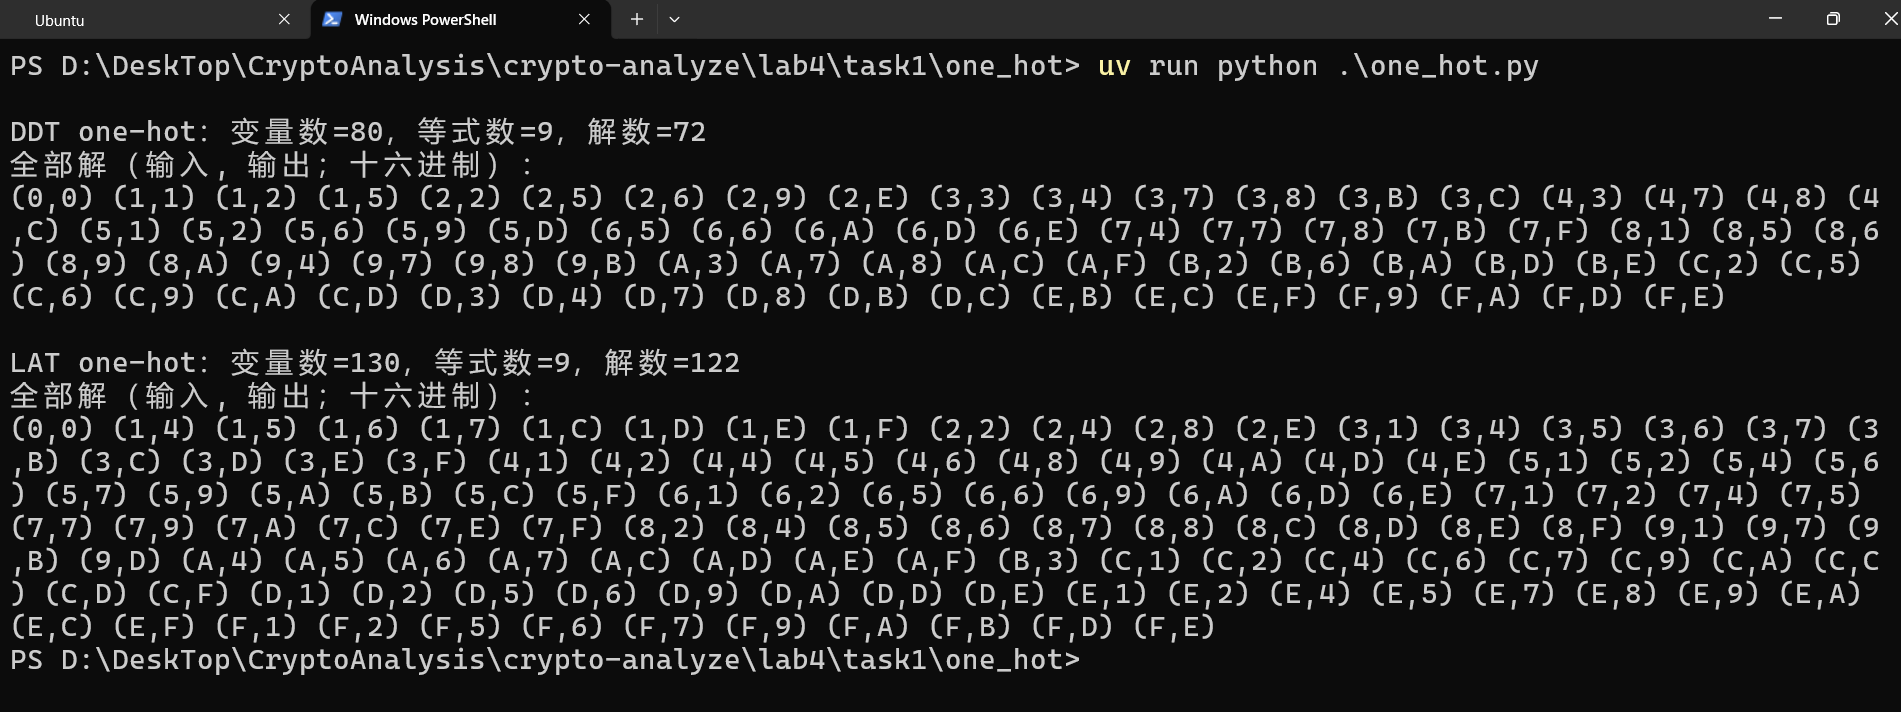
\includegraphics[width=\textwidth]{figures/task1/Grubi_solve1.png}
    \caption{one-hot法的DDT、LAT模型全解枚举结果}
    \label{fig:lab4-task1-one-hot}
\end{figure}

DDT模型有72个选择变量，加上8个原始变量，共$72+8=80$个二进制变量；LAT模型对应$122+8=130$个二进制变量。两者均有9条等式，与上述建模过程一致。求解得到的DDT解数为72，LAT解数为122，按输入分组后与图~\ref{fig:lab4-task1-ddt-lat}各行的非零列逐项相同，说明合法点被完整枚举，零表项对应的点均被排除。
